According to the architecture we have chosen, our system will be composed of these high-level components:
\begin{itemize}
    \item Client-tier components: run on the client machine; these components will be represented as a unique main component in our Component Diagram;
    \item Web-tier components: run on the Java EE server; they are organized in Servlets and JSP pages and they will be used to manage the interaction with the web application;
    \item Business-tier components: run on the Java EE server; these components manage the internal logic of the system and they will be analyzed in the Component Diagram;
    \item Enterprise Information System (EIS)-tier components: run on the database server and handle enterprise infrastructure systems, database systems and legacy systems.
\end{itemize}

The following diagram shows the architectural model of our system, based on the Java EE approach. It also shows how high-level components interact one with the others.

    \begin{figure}[H]
        \centering
        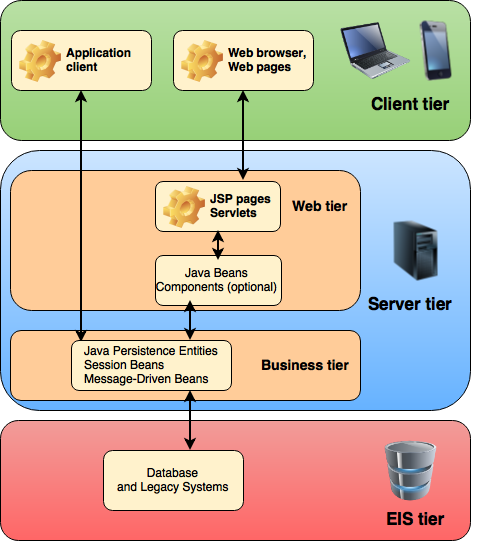
\includegraphics[width=9cm]{./Images/ArchitecturalModel.png}
        \caption{Architectural model of our system}
        \label{architectural-model}
    \end{figure}

As the figure \ref{architectural-model} shows, the business tier is composed of session beans, JPA and message-driven beans. These components will be useful to manage our business logic:
    \begin{itemize}
        \item Session beans: in our system, we will choose stateful beans in order to track the session of a specific user; in this way, a client will be associated to a specific bean during all the session's duration and the bean will be destroyed after the termination of the session.
        \item JPA entities: these entities are associated to Java classes and each of them is mapped to a table in the database; thanks to JPA implementations, it is possible to materialize those entities in the database at runtime.
        \item Message-driven beans: these beans allow our applications to process messages asynchronously; for example, when the client makes a new request, a message is sent to the CallManager component; this process is asynchronous and so the client application can continue doing its tasks, it does not have to wait for the messages to be received and processed. The good thing is that the EJB container will manage all this process. 
    \end{itemize}
In order to explain how logical layers are distributed among the tiers, we have to distinguish into two case: the mobile application and the web one.

\subsubsection{Mobile application}

    \begin{figure}[H]
        \centering
        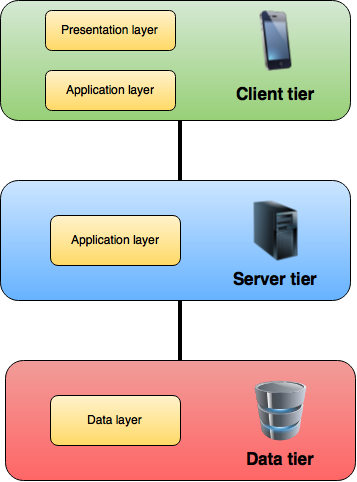
\includegraphics[width=8cm]{./Images/MobileApplication.png}
        \caption{Three-tier architecture for the mobile application}
    \end{figure}

    \begin{itemize}
        \item Client tier: it will implement the presentation layer but also the application layer:  when the client's device will receive from the server JSON data, it will have to parse them and then, according to the business logic, create the view that will be visualized on the device.
        These clients will be not thin because they need to implement part of the application layer, in addition to the presentation layer.
        \item Server tier: it will implement the business logic; this means that this server is in charge to manipulate the data and perform detailed processing. For example, this level will be responsible for managing all the requests from users and changing taxi drivers' status dynamically. 
        \item Data tier: it refers only to the data layer, where all the data of our system will be stored. For example, it will store all the details about requests, taxi drivers' information and so on.
    \end{itemize}

\subsubsection{Web application}

    \begin{figure}[H]
        \centering
        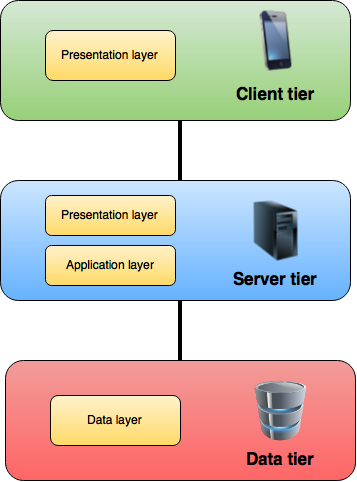
\includegraphics[width=8cm]{./Images/WebApplication.png}
        \caption{Three-tier architecture for the web application}
    \end{figure}
    
    \begin{itemize}
        \item Client tier: it will implement only the presentation layer; in fact, the client's device will receive from the server HTML pages and its main function is to translate those pages so that the user can understand the result. 
        \newline 
        This tier will also have to perform some controls on the users' input (for example it will check if the date of a reservation exists) but, due to the fact that these actions are minimal, we do not consider them as an implementations of the application layer. So, web clients will be thin clients because they will not need to perform complexes business rules.
        \item Server tier: it will implement the business logic and the presentation layer; this means that this server is in charge to create dynamic web pages in HTML and manipulate the data.
        \item Data tier: it refers only to the data layer, where all the data of our system will be stored. For example, it will store all the details about requests, taxi drivers' information and so on.
    \end{itemize}